\documentclass{beamer}
\usepackage[utf8]{inputenc}
\usepackage[croatian]{babel}
\usepackage{helvet}
\usepackage{graphicx}
\usepackage{tikz}
\usepackage{listings}

	\usetikzlibrary{shapes, arrows, positioning}
	\usetheme{Boadilla}
	\usecolortheme{crane}

	\title[TikZ paket]{Izrada grafike koristeći TikZ paket}
	\subtitle{Računalne vještine}
	\author{V. Salamon, K.Pavlović, D.Silić}
	\Institute{Riteh}
	\date

\begin{document}

	\begin{frame}
	\titlepage
	\end{frame}

	\begin{frame}
	\frametitle{Sažetak}
		\begin{itemize}
			\item Vektorska grafika
			\item PGF/TikZ
			\item TikZ
			\item Korištenje TIkZ-a
			\item Dijagrami toka
			\item Definicija okruženja
			\item Korištene naredbe
		\end{itemize}	
	\end{frame}

	\begin{frame}
	\frametitle{Vektorska grafika}
		\begin{itemize}
			\item Koristi dvodimenzionalne poligone za reprodukciju slika u računalnoj grafici
			\item Svaka točka ima određenu poziciju na x i y osi ravnine te određuje put staze
			\item Svakoj stazi je moguće dodijeliti različite atribute poput: boje, oblika, krivulje, debljine i punjenja
			\item Primjer: razmatramo krug radijusa r; podatci koji su potrebni računarskom programu za iscrtavanje tog kruga su:
			\begin{enumerate}
			\item radijus r
			\item koordinatna pozicija središnje točke kruga
			\item stil i boja linije
			\item stil i boja punjenja objekta
			\end{enumerate}	
		\end{itemize}
	\end{frame}

	\begin{frame}
	\frametitle{Prednosti vektorske grafike}
	\begin{itemize}
		\item Prednost vektorske grafike naprema rasterskoj su:
		\begin{enumerate}
		\item manja količina informacija omogućava manju veličinu datoteke
		\item  sve su informacije zapamćene i mogu se kasnije mijenjati; 
    	to znači da kasnije možemo izmjenjivati svojstva slike
    	bez smanjenja kvalitete crteža kao kod rasterkse slike
		\end{enumerate}	
		\end{itemize}
	\end{frame}

	\begin{frame}
	\frametitle{PGF/TikZ}
		\begin{itemize}
		\item TikZ - najsloženiji i najmoćniji alat za stvaranje grafičkih elemenata u LaTeX-u
		\item PGF/TikZ - dva jezika koji rade u paru, služe nam za izradu vektorske grafike pomoću geometrijskog odnosno algebarskog opisa
		\item PGF („Prijenosni grafički format”) - osnovni sloj koji pruža korisniku osnovne naredbe za izradu grafike 
  		\item TikZ - sučelje sa posebnom sintaksom koja olakšava uporabu PGF-a
  		\item PGF je jezik niže razine, dok je TikZ skup makronaredbi na višoj razini koje koriste PGF
  		\end{itemize}	
	\end{frame}	

	\begin{frame}
	\frametitle{TikZ}
		\begin{itemize}
		\item „TikZ ist kein Zeichenprogramm” (TikZ nije program za crtanje)
		\item Dobivamo sve prednosti korištenja TeX-a za grafiku poput:
			\begin{enumerate}
			\item brzog stvaranja jednostavne grafike
			\item korištenje makronaredbi
 			\item precizno pozicioniranje
			\end{enumerate}
		\item Također i nedostatke:	
			\begin{enumerate}
			\item strma krivulja učenja
			\item nema WYSIWYG pristupa rada
 			\item male promjene zahtijevaju dugo vrijeme ponovnog prevođenja
			\end{enumerate}
  		\end{itemize}	
	\end{frame}

	\begin{frame}
	\frametitle{Usporedba sa ostalim grafičkim paketima}
		\begin{itemize}
			\item Usporedba TikZ-a u odnosu na druge pakete:
			\begin{itemize}
			\item standardna LaTeX-ova {picture} okolina nam omogućava izradu jednostavne grafike, ali ništa više od toga - rezultat portabilnosti {picture} okoline. Ne radi s pdftexom niti s bilo kojim drugim upravljačkim programom koji ne proizvodi ništa drugo osim PostScript koda.
  			\item Xypic je nešto stariji paket za izradu grafike. Nešto teži za uporabu i općenito učenje jer je njegova sintaksa, moglo bi se reći, kriptirana.
  			\item Dratex paket je vrlo mali paket za izradu grafike. U usporedbi sa TikZ-om i ostalim paketima je vrlo malen što može, a i ne mora biti njegova prednost.
  			\item Metapost je program koji je vrlo moćna alternativa TikZ-u. Prije je bio zaseban program što je prouzročilo mnogo problema, no sada je ugrađen unutar LaTeX-a.
  			\item Xfig program je važna alternativa TikZ-u za korisnike koji ne žele "programirati" svoju grafiku kao što je to potrebno uz TikZ i ostale navedene pakete. Postoji program koji pretvara xfig grafiku u TikZ.
  			\end{itemize}
  		\end{itemize}	
	\end{frame}	

	\begin{frame}
	\frametitle{Dijagrami toka u Tikz-u}
		\begin{itemize}
		\item Jedna od mnogih stvari za koje možemo upotrebljavati Tikz okruženje u latex uređivaču je svakako i izrada dijagrama toka.
		\item Dijagrame toka korištenjem  Tikz-a izrađujemo pomoću raznih elemenata predefiniranih unutar samoga okruženja te njegovih raznih biblioteka.
  		\end{itemize}	
	\end{frame}

	\begin{frame}
	\frametitle{Dijagrami toka u Tikz-u}
		\begin{figure}
			\begin{center}
				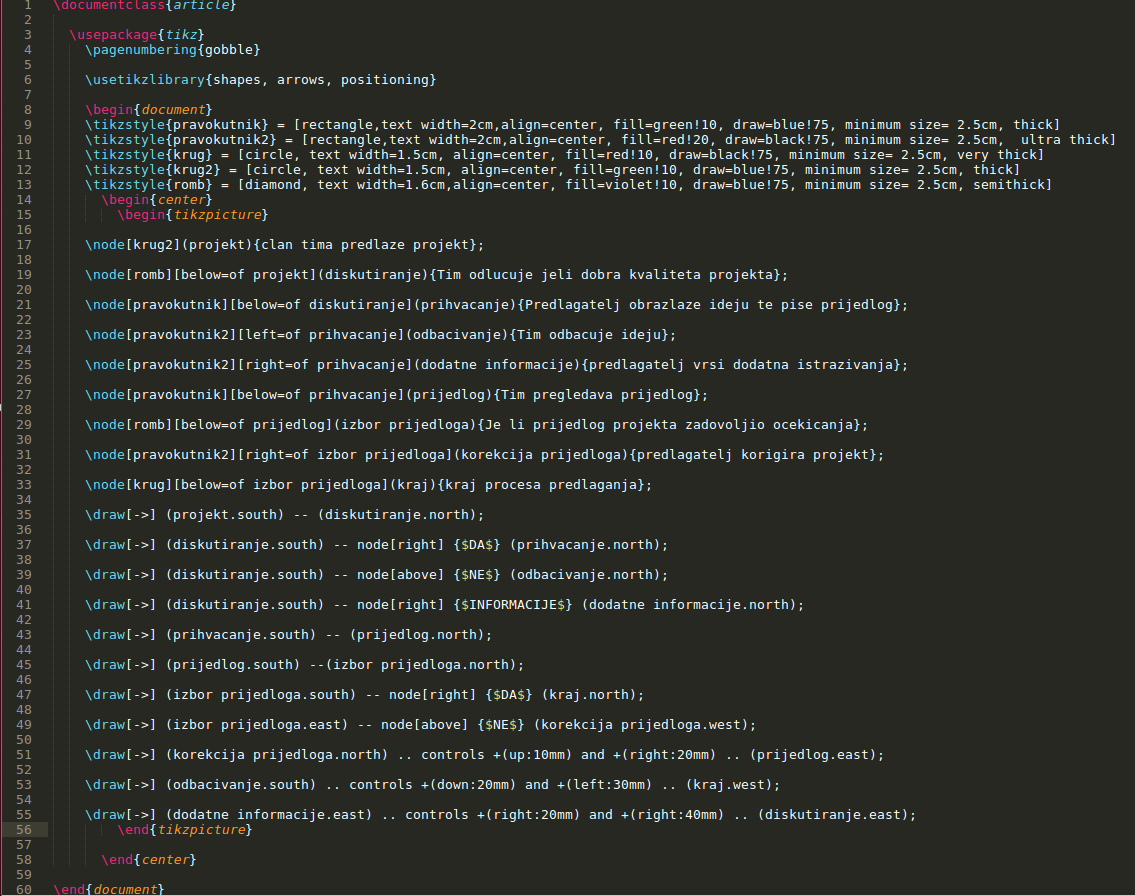
\includegraphics[width=12 cm,height=7cm]{kod.png}
				\caption{Kod dijagrama toka}
			\end{center}
		\end{figure}
	\end{frame}

	\begin{frame}
	\frametitle{Dijagrami toka u Tikz-u}
	\begin{figure}
		\begin{center}
			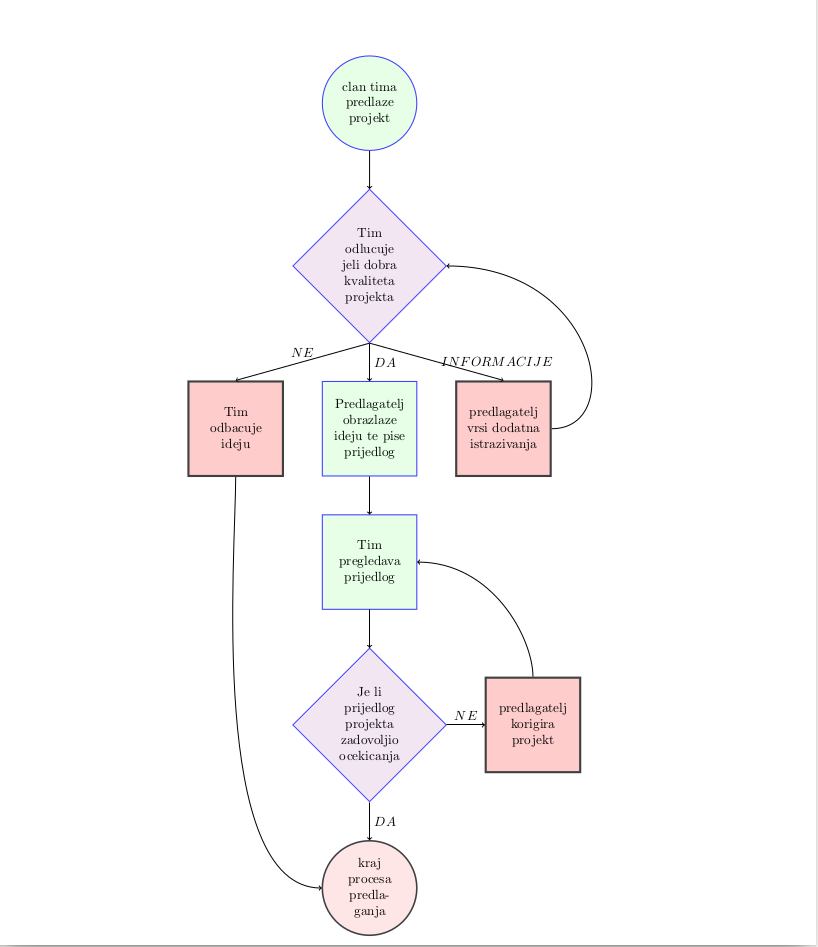
\includegraphics[width=12 cm,height=7cm]{izgled.png}
			\caption{Izgled dijagrama toka}
		\end{center}
	\end{figure}
	\end{frame}


\begin{frame}[fragile]
	\frametitle{Preambula Tikz dokumenta}
		\begin{itemize}
		\item  Na početku izrade dijagrama u preambuli dokumenta potrebno je deklarirati kako se radi o paketu naredbi Tikz pomoću naredbe\begin{verbatim}\usepackage{tikz}\end{verbatim}
		\item \begin{verbatim}\usetikzlibrary{shapes, arrows, positioning}\end{verbatim}
		\item Neke od najčešće korištenih biblioteka su:
			\begin{enumerate}
				\item arrows – koristi se za crtanje različitih vrsta strelica
				\item backgrounds – koristi se za definiranje različitih pozadina slika
				\item chains – služi za lakše poravnavanje grafičkih elemenata u dokumentu
				\item shapes – Jedna od najbitnijih biblioteka Tikz-a koja služi za definiranje različitih geometrijskih elemenata kao i raznih drugih oblika 
			\end{enumerate}
		\item Biblioteke koje smo koristili pri izradi dijagrama toka u primjeru su:
			\begin{enumerate}
				\item shapes – upravo zbog mogućnosti crtanja različitih geometrijskih oblika koji su nam biti pogodni u izradi dijagrama.
				\item arrows – kako bismo mogli povezati nacrtane objekte
				\item positioning – kako bismo mogli slagati elemente u određene odnose jedan naprema drugom 
			\end{enumerate}
  		\end{itemize}	
\end{frame}

\begin{frame}[fragile]
	\frametitle{Preambula Tikz dokumenta}
		\begin{itemize}
		\item \begin{verbatim}\tikzstyle{romb} = [diamond, text width=1.6cm,
		align=center,fill=violet!10, draw=blue!75,
		minimum size= 2.5cm,semithick]\end{verbatim}
		\item Pomoću ove naredbe predefiniramo procesoru kako će izgledati pojedini objekt kojega ćemo kasnije moći jednostavno pozvati pomoću dodjeljene oznake
		\item Opcije koje smo u konkretnom primjeru koristili:
			\begin{enumerate}
				\item diamond – označava kako se radi o obliku romba odnosno dijamanta
				\item text width=1.6cm – označava kako će širina teksta biti 1.6 cm
				\item align=center – tekst unutar objekta će biti centralno poravnat
				\item fill=violet!10 – označava kako će objekt biti ispunjen ljubičastom bojom kojoj će intenzitet biti 10% 
				\item draw=blue!75 – obrubljuje objekt sa crtom plave boje intenziteta 75%
				\item minimum size=2.5cm – označava kako minimalna veličina tog elementa mora biti 2.5cm
				\item semithick – označava debljinu crte obruba elementa
			\end{enumerate}
  		\end{itemize}	
\end{frame}

\begin{frame}[fragile]
	\frametitle{Definicija okruženja}
		\begin{itemize}
		\item Nakon što smo definirali objekte koje ćemo koristiti potrebno je definirati okruženje u kojem ćemo raditi.
		\item Dekaraciju okruženja vršimo naredbom \begin{verbatim}\begin{tikzpicture}\end{verbatim}
		\item Glavna naredba koju ćemo koristiti, a koja će nam poslužiti upravo zbog svoje svestranosti je naredba \begin{verbatim}\node\end{verbatim} 
		\item Druga naredba koju ćemo koristiti kako bismo povezali napravljene objekte je naredba \begin{verbatim}\draw\end{verbatim}
  		\end{itemize}	
\end{frame}

\begin{frame}[fragile]
	\frametitle{node naredba}
		\begin{itemize}
		\item \begin{verbatim}\node[pravokutnik2][left=of prihvacanje](odbacivanje){Tim
		odbacuje ideju};\end{verbatim}
		\item Node se tipično koristi kada se radi o nekom jednostavnom obliku koji u sebi može i ne mora sadržavati neki tekst,a u najjednostavnijem slučaju označava neki tekst koji je postavljen na određenu koordinatu.
		\item U slučaju iz primjera koristit ćemo node element kako bismo pozvali oblike koje smo prethodno deklarirali
		\item U prvoj uglatoj zagradi pišemo ime deklariranog elementa kojega želimo pozvati
		\item Drugu uglatu zagradu koristimo kako bismo definirali odnos između trenutnog i njemu susjednog elementa
		\item Oblim zagradama definiramo ime objekta
		\item U uglate zagrade stavljamo tekst koji želimo da se pojavi u objektu
  		\end{itemize}	
\end{frame}

\begin{frame}[fragile]
	\frametitle{draw naredba}
		\begin{itemize}
		\item \begin{verbatim}\draw[->] (projekt.south) -- (diskutiranje.north);\end{verbatim}
		\item draw naredbu isto je tako moguće koristiti u mnogim primjenama
		\item U ovom primjeru koristit ćemo je kako bismo strelicama spojili stvorene objekte
		\item Uglata zagrada nam pokazuje o kakvoj se strelici radi 
		\item U oblim zagradama specificiramo koje objekte povezujemo te kako ih povezujemo
		\item Dodatkom node elementa moguće je dodati tekst u strelicu 
		\item naredbom controls možemo mijenjati izgled strelice
  		\end{itemize}	
\end{frame}

\begin{frame}[fragile]
	\frametitle{Zatvaranje okruženja}
		\begin{itemize}
		\item Kada smo završili sa deklaracijom svih elemenata preostaje nam još samo zatvoriti Tikz okruženje
		\item Zatvaranje vršimo naredbom \begin{verbatim}\end{tikzpicture}\end{verbatim}
  		\end{itemize}	
\end{frame}	

\begin{frame}[fragile]
	\frametitle{Struktura stabla}
		\begin{itemize}
		\item Struktura stabla jedan je od najčešćih načina vizualizacije hijararhijske strukture
		\item Struktura stabla omogućuje nam postavljanje elemenata u takozvani roditeljski odnos gdje svaki element roditelj(parent) može imati mnogo pod elemenata koji se nazivaju djeca(child)
  		\end{itemize}	
\end{frame}	

\begin{frame}[fragile]
	\centering
	\frametitle{Jednostavna stabla}
	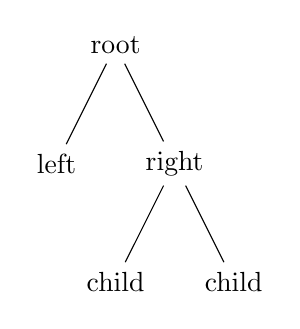
\begin{tikzpicture}
		\node {root}
			child {node {left}}
			child {node {right}
				child {node {child}}
				child {node {child}}
		};
	\end{tikzpicture}
	\begin{itemize}
	\item \begin{verbatim}
		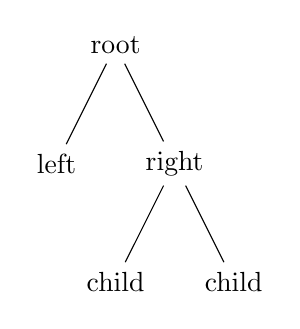
\begin{tikzpicture}
		\node {root}
		 child {node {left}}
		 child {node {right}
		  child {node {child}}
		  child {node {child}}
		};
	\end{tikzpicture}
	\end{verbatim}
	\end{itemize}
\end{frame}	

\begin{frame}[fragile]
	\frametitle{Naredbe stabla}
		\begin{itemize}
		\item kao i u primjerima od prije osnovna naredba za pokretanje strukture bit će naredba\begin{verbatim}\node {root}\end{verbatim}
		\item kako bismo kreirali podelemente koristimo naredbu 
		\begin{verbatim}child {node {left}}\end{verbatim} svaki dodani element moguće je dalje dijeliti na manje dijelove tipkom tab
		\item I ovdje je moguće unaprijed definirati postavke prikazivanja stabla naredbom
		\begin{verbatim}\tikzstyle{level 1}=[sibling distance=8mm]\end{verbatim}
		\end{itemize}	
\end{frame}	
\end{document}
 
